%Most of the material presented in this Section is not original, we use it mainly as
%a reminder and an opportunity to present quantities and notations that will be
%used later on.
\color{blue}
\begin{itemize}
\item J'ai renomme "model" en "formulation". Le premier designe plutot le modele moyenne a deux fluides.
\item la definition du dirac interfacial etait totalement bancale ... fait attention a ce genre de point de detail cela discredite ton propos.
\item il faut definir les normales.
\item il me semble qu'il faudrait plus mettre en valeur l'originalite ici, c'est de bien ecrire les relations de saut dans la formulation a deux fluides (a discuter ensemble.).
\end{itemize}
\color{black}
%\tb{}
In this section we derive the conservation equations using a two-fluid formulation.%the two-fluid formulation of the balance equations. %derive the equations governing the two fluid motion.
%the two-fluid model. 
While the derivation of this formulation is available in various studies such as those by \citet{kataoka1986local,lhuillier2010multiphase,ishii2010thermo,morel2015mathematical} our approach here enables us to introduce specific notations and key results that will prove useful for later discussions. %Although the derivation of the two fluid model may be found in many other studies \citep{lhuillier,ishii,morel,delhaye} this derivation allows us to present the notations and some results which will be usefull later on. %starting from 
\begin{figure}[h!]
    \centering
    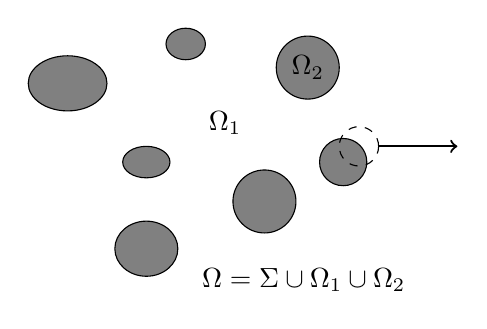
\begin{tikzpicture}
        \foreach \x/\y/\ra/\r in {
        1/3/0.2/0.25,
        2.55/2.7/0.4/0.4,
        0.5/0.4/0.35/0.4,
        2/1/0.4/0.4,
        3/1.5/0.3/0.3,
        0.5/1.5/0.2/0.3,
        -0.5/2.5/0.35/0.5}{
            \draw[fill=gray](\x,\y) ellipse(\r cm and \ra cm);
        }
        \draw[dashed](3.2,1.7)circle(0.25);
        % \draw[thick,->](3.2,1.7)++(0.1767,0.1767)--++(0.4,0.4)--++(1,0);
        \draw[thick,->](3.2,1.7)++(0.25,0)--++(1,0);
        \draw(2.55,2.7)node{$\Omega_2$};
        \draw(1.5,2)node{$\Omega_1$};
        \draw(2.5,0)node{$\Omega = \Sigma \cup \Omega_1 \cup \Omega_2$};
        % \draw(2.5,-1)node{$\Sigma = \sum_\alpha \Sigma_\alpha$};
        % \draw(2.5,-0.5)node{$\Omega_2 = \sum_\alpha \Omega_\alpha$};
    \end{tikzpicture}
    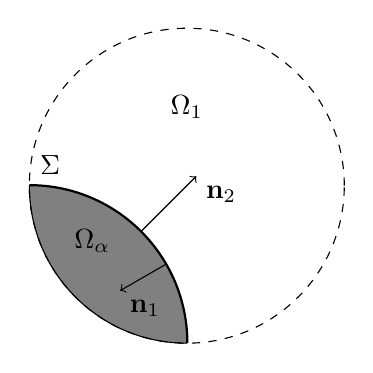
\begin{tikzpicture}%[scale = 0.9]
        \draw[very thick](0:2)arc(0:90:2)node[above right]{$\Sigma$};
        \draw[fill=gray](0:2)arc(0:90:2)arc(180:270:2);
        \draw[dashed](2,2)circle(2);
        \draw[->](1.42,1.42)--++(0.7,0.7)node[below right]{$\textbf{n}_2$};
        \draw[->](1.73,1)--++(-0.577,-0.333)node[below right]{$\textbf{n}_1$};
        \draw(2,3)node{$\Omega_1$};
        \draw(0.8,1.3)node{$\Omega_\alpha$};
    \end{tikzpicture}
    \caption{Topology of dispersed two-phase flows.}%Domain definitions and scheme of the topology of dispersed two-phase flows.}
    \label{fig:Scheme}
\end{figure}

We consider a system consisting of two phases, separated by a sharp interface $\Sigma(t)$ which evolves over time. For further insights into the modeling of sharp interface thermodynamics, a comprehensive review may be found in \cite{bothe2022sharp}. %you can refer to the comprehensive review by Bothe et al. (2022).
%More details on the modeling of a sharp interface thermodynamics may be found in the recent review of \cite{bothe2022sharp}.
Each phase subdomain is denoted as $\Omega_1(t)$ and $\Omega_2(t)$, representing the continuous phase (1) and the dispersed phase (2) respectively (refer to Figure \ref{fig:Scheme}).
%Each phase subdomain is denoted $\Omega_1(t)$ and $\Omega_2(t)$ for the continuous phase ($1$) and the dispersed phase ($2$) respectively (see \ref{fig:Scheme}). 
%The mathematical and physical definition of $\Sigma(t)$ is by no means straightforward, therefore, the interested reader is refereed to \cite{bothe2022sharp} to have a deeper understanding of sharp interface modeling. 
The entire domain, denoted as $\Omega$, is defined as the union of $\Omega_1$, $\Omega_2$, and $\Sigma$.
To track the position of the phase indexed $k$ and the interfaces, we introduce the phase indicator function $\chi _k$ defined as
\begin{align}
    \chi_k(\textbf{x},t) =  \left\{
      \begin{tabular}{cc}
        $1 \;\text{if} \;\textbf{x} \in \Omega_k(t)$\\
        $0 \;\text{if} \;\textbf{x} \notin \Omega_k(t)$
      \end{tabular}
      \right.
      \text{for $k = 1,2$}.
    %   \label{eq:PIF}
%    && \delta_I(\textbf{x},t) =  \left\{
%      \begin{tabular}{cc}
%        $1 \;\text{if} \;\textbf{x} \in \Sigma(t)$\\
%        $0 \;\text{if} \;\textbf{x} \notin \Sigma(t)$
%      \end{tabular}
%      \right.,
      \label{eq:PIF}
\end{align}
 % and the interface indicator function $\delta _I$ as
To enhance clarity, we will omit the time and position parameters from $\chi_k(\textbf{x},t)$ %and $\delta_I(\textbf{x},t)$
 in the subsequent sections.
%For clarity, we omit the time and position arguments of $\chi_k(\textbf{x},t)$ and $\delta_I(\textbf{x},t)$ in the following sections. 


\subsection{Topological equations}
\color{blue} 
\begin{itemize}
\item Attention il y a un probleme dans ta macro ref quand tu cites plusisurs equations, cela fait equation 1, equation 2, equation 3... alors qu'il faut simplement faire equations (1) (2) and (3)
\item Pour les deux premieres equations ca me va de citer Drew. Par contre pour les deux secondes, Lhuillier et Marle me paraissent plus appropries que Morel (qui les cite juste non ?). Il faut citer les bons auteurs. J'ai trouve un papier qui fait un etat des lieux tres recent dans ce cadre (On the evolution equations of interfacial variables in two-phase flows - IJMF 2023). Ce serait bien de donner quelques details pr passer de 2.2 (pr 2.2 c'est assez connu il me semble donc pas besoin de le montrer) à 2.4, juste dire qu'on prends le gradient n'est pas suffisant (cf les dits papiers). Ca peut etre mis en annexe, ou alors on admets simplement le resultat.
\item concernant 2.5 je ne vois sa trace nulle part dans les papiers cites plus haut. Meme si elle semble etre exacte je la trouve ambigue pr 2 raisons. La premiere est que je n'aime guere la notation $\cdot$ pr designer un produit matrice vecteur. D'une part ce n'est pas un produit scalaire et d'autre part on ne sait jamais sur quel indice on doit faire la sommation. La seconde est que $\mathbf{n}$ n'est pas definie, et si on la definie elle aura un caractere arbitraire ($\mathbf{n}_1$ ou $\mathbf{n}_2$ ?). Je privilegierai donc l'expression suivante:

\begin{equation}
    \grad\delta_I 
    = (\grad \textbf{n}_k)\textbf{n}_k \delta_I + (\grad \delta_I \cdot \textbf{n}_k) \textbf{n}_k \nonumber
\end{equation} 
\item on en avait deja discuté mais je trouve la notation $\divI$ pas tres heureuse car il existe une infinite de vecteur // à une surface. Il semble que seul Bothe l'utilise. Je preferai $\nabla _s$ qui est bcp plus repandue (Lhuillier, Morel, Jacques, Stone, Nadim, ...). Ce serait bien d'ailleurs de le definir plus formellement.
%\item dans 2.5 de quel $n$ parle on ? le 1 ou 2 ? c
\end{itemize}
\color{black}
Using the distribution formalism, one may show that $\chi_k$ obeys the following relations \citep{drew1983mathematical} %from \ref{eq:PIF} 

%the transport equation of $\chi_k$ from \ref{eq:PIF} obey the following relations \citep{drew1983mathematical} 
\begin{align}
    \pddt \chi_k
    + \textbf{u}_I^0 \cdot \grad \chi_k
    &= 0,
    \label{eq:dt_chi_k}\\
% \end{align}
% \begin{align}
    \label{eq:grad_chi_k}
    \grad \chi_k
    &= - \delta_I \textbf{n}_k. 
\end{align}
where $u^0_I$ is the velocity of the interface and $\delta_I$ is the Dirac function localized on the interface.
Then, to describe the evolution of $\delta_I$ we take the gradient of \ref{eq:dt_chi_k} and the gradient of \ref{eq:grad_chi_k} which yields two equations of the interface indicator function \citep{morel2007surface},
% \begin{equation}
%     \pddt \delta_I
%     + \div \left[(\textbf{u}_I^0\cdot\textbf{n})\textbf{n} \delta_I\right]
%     = \delta_I (\textbf{u}_I^0\cdot\textbf{n})(\div\textbf{n}),
% \end{equation}
% where we did not specify the index of \textbf{n} since it appears twice in all terms of the equation. 
% As pointed out by \citet{morel2007surface}, it is more convenient to rewrite this equation under the following form,
\begin{align}
    \pddt \delta_I
    + \div (\delta_I \textbf{u}_I^0)
    &= \delta_I \divI \textbf{u}_I,
    \label{eq:dt_delta_I}\\
% \end{align}
% Lastly, we derive an expression for the gradient of $\delta_I$ by taking the gradient of \ref{eq:grad_chi_k}, resulting in,
% \begin{align}
    \grad\delta_I 
    &= \textbf{n} \cdot \grad (\textbf{n} \delta_I),
    \label{eq:grad_delta_I}
\end{align}
where $\divI$ is the surface divergence operator. \ref{eq:dt_chi_k}, \ref{eq:dt_delta_I}, \ref{eq:grad_delta_I} and \ref{eq:grad_chi_k} are commonly referred to as the topological equations as it describe the evolution in space and time of the topology.

%\section{General conservation  equations}
\subsection{Local conservation equations}
\color{blue} 
Partie a retravailler:
\begin{itemize}
\item je n'aime pas trop la premiere equation integrale. Cela me parait bcp plus physique de decomposer les grandeurs des le debut en une partie dans le volume et une partie surfacique et d'écrire l'equation integrale sur l'ensemble de ces quantité comme le fait Bothe ou Slattery.
\item Essaye d'etre precis quand tu fais ton bilan : est ce un volume de controle materiel ou un volume non-materiel fixe ? vu que tu prends en compte les flux au travers de sa surface cela semble etre un volume non-materiel. A rediscuter ensemble
\item j'ai l'impression que notations ne sont pas coherentes. Il manque l'indice $0$, le terme source petit s devient grand S, ...
\item pour l'instant je n'ai pas relu en detail cette section
\end{itemize}
\color{black}
\begin{figure}[h]
    \centering
    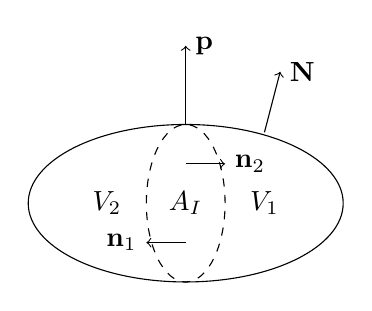
\begin{tikzpicture}
        \draw (0,0) ellipse (2 and 1);
        \draw[dashed] (0,0) ellipse (0.5 and 1)node{$A_I$};
        \draw[->](0,1)--++(0,1)node[right]{\textbf{p}}; 
        \draw[->](1,0.9)--++(0.2,0.77)node[right]{\textbf{N}}; 
        \draw[->](0,-0.5)--++(-0.5,0)node[left]{$\textbf{n}_1$}; 
        \draw[->](0,0.5)--++(0.5,0)node[right]{$\textbf{n}_2$}; 
        \draw (1,0)node{$V_1$};
        \draw (-1,0)node{$V_2$};
    \end{tikzpicture}
    \caption{Scheme of an arbitrary material control volume.   }
\end{figure}

Let $f^0$  be an arbitrary quantity to be conserved. 
Then $\bm\Phi^0$ refer to the non-convective flux of $f^0$. 
Then $s^0$ refer to source term  related to  $f^0$. 
Then, for an arbitrary control volume we have, 
\begin{equation*}
    \ddt \int_{V} f^0 dV 
    = 
    \int_{V} s^0 dV 
    + \int_{\partial V} \mathbf{\Phi}^0 \cdot \textbf{N} dS,
\end{equation*}
where $\textbf{N}$ is the normal of the control volume. 
Any quantities defined in $V_k$ will be noted with a subscript $_k$ and those who are defined at the interface with $_I$. 
Therefore, if we decompose any quantity such as $f^0 = \sum_k f_k^0 \chi_k + f_I^0 \delta_I$ we obtain, 
\begin{multline*}
    \sum_k\left[\ddt \int_{V_k} f_k^0 dV 
    - \int_{V_k} s_k^0 dV 
    - \int_{A_k} \mathbf{\Phi}_k^0 \cdot \textbf{N} dS
    \right]
    + \ddt \int_{A_I} f_I^0 dS 
    - \int_{A_I} s_I^0 dS 
    - \int_{C} \mathbf{\Phi}_I^0 \cdot \textbf{p} dC 
    = 0
\end{multline*}
Using the Reynolds transport theorem on volume integral yields,
\begin{align*}
    \ddt \int_{V_k} f_k^0 dV 
    &= \int_{V_k} \pddt f_k^0 dV 
    + \int_{A_I \cup A_k} f_k^0 \textbf{u} \cdot \textbf{n}_k dS\\
    &= \int_{V_k} \left[
        \pddt f_k^0  + \div (f_k^0 \textbf{u}_k^0) 
    \right]dV 
    + \int_{A_I} f_k^0 (\textbf{u}_I^0 - \textbf{u}_k^0) \cdot \textbf{n}_k dS\\
\end{align*}
where $\textbf{n}_k$ is the normal of the interface $A_I$ on the outward direction of the $k$ phase. 

The second term is integrated only over $A_I$ as it is the interface between both phase and not the one of the control volume. 
Using the Ledbiz rule for integration on surface yields, 
\begin{align*}
    \ddt \int_{A_I} f_I^0 dS 
    &= \int_{A_I} \left[
        \pddt f_I^0  + \divI (f_I^0 \textbf{u}_I^0) 
    \right]dS
\end{align*}

Regarding the non-convective integrals, by using the divergence theorem we can write\citep{nadim1996concise}, 
\begin{align*}
    \int_{A_k} \mathbf{\Phi}_k^0\cdot \textbf{n}_k dS
    = \int_{V_k} \div\mathbf{\Phi}_k^0 dV
    - \int_{A_I} \mathbf{\Phi}_k^0\cdot \textbf{n}_k dS. 
\end{align*}
The last term can also be re-written with the divergence theorem \citet{nadim1996concise},
\begin{align*}
    \int_{C} \mathbf{\Phi}_I^0\cdot \textbf{p} dC 
    = \int_{A_I} \divI \mathbf{\Phi}_I^0 dS
    - \int_{A_I} \mathbf{\Phi}_I^0 \cdot \textbf{n} \div \textbf{n} dS
\end{align*}
Notice that whether it is $\textbf{n}_1$ or $\textbf{n}_2$ the second term on the left conserve the same sign. 

Taking in account these reformulations, we can re-write the integral balance previously exposed by, 
\begin{align*}
    \sum_k \int_{V_k}{\left[
        \pddt f_k^0
        + \div (f_k^0\textbf{u}_k^0 - \bm\Phi_k^0)
        - s_k^0
    \right]}\\
    + \sum_k\int_{A_I}{\left[
        f_k^0(\textbf{u}_I^0 - \textbf{u}_k^0)
        + \bm\Phi_k^0
    \right]\cdot \textbf{n}_k}
    + \int_{A_I}{\left[
        \pddt f_I^0 
        + \divI (f_I^0 \textbf{u}_I - \bm\Phi_I^0)
        + \bm\Phi_I^0 \cdot \textbf{n} \div \textbf{n}
    \right]} =0 
\end{align*}

Every integral of volume must be balanced independently of the surface integral. 
This means that we can separate this equation into two, 
\begin{equation*}
    \pddt f_k  
    + \div (f_k \textbf{u}_k - \mathbf{\Phi}_k) 
    =\textbf{S}_k. 
\end{equation*}
\begin{equation}
    \pddt f_I  
    + \divI (f_I \textbf{u}_I -\mathbf{\Phi}_I)
    + \mathbf{\Phi}_I \cdot \textbf{n} \div \textbf{n}
    = 
    + \textbf{S}_I
    - \sum_k \left[
    f_k (\textbf{u}_I - \textbf{u}_k)
    + \mathbf{\Phi}_k
    \right] \cdot \textbf{n}_k. 
    \label{ap:eq:dt_f_I}
\end{equation}
These equations are valid in $\Omega_k(t)$ and $\Sigma(t)$ for volume and surface quantity, respectively. 

Now let's reformulate the third term of the surface balance equation. 
Let $\textbf{F}$ be an arbitrary surface quantity. 
It can be split into two part such as, 
\begin{equation*}
    \textbf{F} 
    = \textbf{F} \cdot \textbf{n}\textbf{n}
    + (\textbf{I} - \textbf{nn})  \cdot \textbf{F}
    = \textbf{F}_\bot + \textbf{F}_{||}.
\end{equation*}
Injecting this decomposition inside the Gauss theorem on an arbitrary control volume it can be shown that, 
\begin{equation*}
    \int_{S} \divI \textbf{F}dS
    = 
    \int_{S} \left[\divI \textbf{F}_{||} 
    + \textbf{F} \cdot \textbf{n} \div\textbf{n}
    \right]dS
\end{equation*}
Consequently, we have the following relation,
\begin{equation*}
    \int_{A_I} \divI \bm\Phi_I^0dS
    = 
    \int_{A_I} \left[\divI \bm\Phi_{I||}^0
    + \bm\Phi_I^0 \cdot \textbf{n} \div\textbf{n}
    \right]dS
\end{equation*}

By taking in account this relation it is easy to take or not the normal components of a vector to the interface within the balance equaitons. 
For example, we can write either, 
\begin{equation}
    \pddt f_I  
    + \divI (f_I \textbf{u}^I_{||} -\mathbf{\Phi}^I_{||})
    + f_I \textbf{u}_I \cdot \textbf{n} \div \textbf{n}
    - \textbf{S}_I
    = 
    - \sum_k \left[
    f_k (\textbf{u}_I - \textbf{u}_k)
    + \mathbf{\Phi}_k
    \right] \cdot \textbf{n}_k 
    \label{ap:eq:dt_f_I2}
\end{equation}
Or 
\begin{equation}
    \pddt f_I  
    + \divI (f_I \textbf{u}^I -\mathbf{\Phi}^I_{||})
    - \textbf{S}_I
    = 
    - \sum_k \left[
    f_k (\textbf{u}_I - \textbf{u}_k)
    + \mathbf{\Phi}_k
    \right] \cdot \textbf{n}_k 
    \label{ap:eq:dt_f_I2}
\end{equation}
where we have changed the flux term formulation. 
\tb{Daniel prefer la formulation 1 car elle fait apparaitre la vitesse normal a l'interface est les fluxs sont des "vrai" fluxs dans le plan 2D}

\tb{
    Meme si c'est moins physique ici on prefere la 2) car elle est plus compact 
}


% Using the distribution formalisum together with the Reynolds transport theorem we may write that this equation :
% \begin{equation*}
%     \ddt \int_{V} f^0 dV 
%     =
%     \int_{V} \left[
%         \pddt f^0  + \div (f^0 \textbf{u}^0) 
%     \right]dV 
%     = 
%     \int_{V} s^0 dV 
%     + \int_{\partial V} \mathbf{\Phi}^0 \cdot \textbf{N} dS,
% \end{equation*}
% In the sens of distribution we know that the derivative of a generalized function $f^0$ can be written \citep{appel2007mathematics}, 
% \begin{equation}
%     \grad f^0 = \sum_k \chi_k \grad f^0_k 
%     + \delta_I (f^0_2 - f^0_1) \textbf{n}_1
% \end{equation}
% and in general we can decompose any function with $f^0 = \sum_k \chi_k f^0_k + \delta_I f_I^0$. 
% Therefore, we can re write the previous equation such that,
% \begin{equation*}
%     \int_{V} \pddt(\sum_k \chi_k f^0_k + \delta_I f_I^0) 
%     + \div(f^0_k \textbf{u}_k^0)
%     dV 
%     = 
%     \int_{V} (\sum_k \chi_k s^0_k + \delta_I s_I^0) dV 
%     + \int_{\partial V} (\sum_k \chi_k f^0_k + \delta_I f_I^0) \cdot \textbf{N} dS,
% \end{equation*}


\subsection{Local conservation equations}
\label{sec:local_eq}
\tb{
\begin{itemize}
\item il faudra enlever cette section car elle est redondante avec celle d'avant. Pour l'instant je l'ai laissé pour avoir le set d'equation sous les yeux c'est plus simple.
\item il faut faire un choix entre la notation $\sum$ et $\Jump{}$. Dans lequation 2.10 quel normal utilise on pour le dernier terme ? j'imagine que c'est une normale arbitraire, mais cf phrase dvan je trouve que cela induit de la confusion avec le symbole $\Jump{}$ en plus. J'ai donc remplacé par la sommation que je trouve bcp plus claire et qui semble plus repandu dans la litteraure (Kataoka, Morel, ...).
%\item pour moi on a pas besoin d'introduire le momentum ici. On en discutera ensemble mais pour l'instant je resterai tres general et je ne m'interesserai qu'à l'applciation en dernier. -> en fait si il faut la definir car on en aura besoin nottament pr certain theoreme lagrangien
\item ne devrait on pas ecrire $\rho _k^0$ en toute generalite ?
\item il faut decrire comment on obtient les equations de conservation de la masse et de qdm sur la surface. D'ailleurs on n'a peut etre pas besoin de la conservation de la masse.
\item pourquoi a on un terme de diffusion de masse pour une interface ? cela me smble incorrect a discuter ensemble
\end{itemize}
}

%Each conservation equation presented above have the same mathematical structure. 
%In the perspective of manipulating these equations it is useful to introduce a generic formulation on which we will carry the derivation.
%For purpose of generality we make no assumption in this general formulation. 
%For example the phase transfer terms will be kept, i.e. $\textbf{u}_I \neq \textbf{u}_k$. 

Let $f_k^0(\textbf{x},t)$ denote a volumetric quantity of arbitrary tensorial order defined in $\Omega_k(t)$.
Likewise, let $f_I^0(\textbf{x}_I,I)$ represent an arbitrary surface property defined on $\Sigma(t)$.
Using the strategy outlined in \citep{bothe2022sharp,morel2015mathematical,slattery2007interfacial}, we can derive the local conservation equations for both $f_k^0(\textbf{x},t)$ and $f_I^0(\textbf{x}_I,t)$, that is,  
\begin{align}
    \label{eq:dt_f_k}
    \pddt f_k^0
    +\div \left(
        f_k^0\textbf{u}_k^0
        - \mathbf{\Phi}_k^0
        \right)
    &= 
    s_k^0
    & \text{ in } \Omega_k(t),&\\
    \pddt f_I^0 
    +\divI
    (
        f_I^0 \textbf{u}_I^0
        - \mathbf{\Phi}_{I||}^0 
    )
    &= 
    s_I^0
    - \sum_k \left[
    f_k^0 (\textbf{u}_I^0 - \textbf{u}_k^0)
    + \mathbf{\Phi}_k^0
    \right] \cdot \textbf{n}_k 
    %- \Jump{
    %    f_k (\textbf{u}_I^0 - \textbf{u}_k^0)
    %    + \mathbf{\Phi}_k^0
    % } 
    & \text{ on } \Sigma(t),&
    \label{eq:dt_f_I}
\end{align}
respectively.
The tensors $\mathbf{\Phi}_k^0(f_k)$ and $\mathbf{\Phi}_{I||}^0(f_I)$ represent the non-convective fluxes corresponding to $f_k^0$ and $f_I^0$. 
Notice that $\mathbf{\Phi}_{I||}^0$ also carries the $_{||}$ subscript which implies that only the tangential component of this tensor remain in the surface balance equation. 
Similarly, $s_k^0(f_k^0)$ and $s_I^0(f_I^0)$ represent the source terms of $f_k^0$ and $f_I^0$, respectively.
Notice, that in \ref{eq:dt_f_I} we kept the mass transfer term $f_k (\textbf{u}_I^0 - \textbf{u}_k^0)$ for purpose of generality. 
It is important to note that \ref{eq:dt_f_k} and \ref{eq:dt_f_I} are solely defined within $\Omega_k(t)$ and $\Sigma(t)$, respectively.
This was also the case for the equations presented in the last two subsections. 
Consequently, these equations are referred to as local conservation equations. This conservation equations may be easily to mass and momentum balance. %\tb{Mettre momentum + C d masse}
Within phase $k$, we note $\rho_k$ the density and $\textbf{u}_k^0$ the local velocity. For mass balance $f_k^0 = \rho_k$, $\mathbf{\Phi}_k^0(f_k) = \mathbf{0}$ and $s_k^0=0$. For momentum balance, $f_k^0 = \rho_k \mathbf{u}_k$, $\mathbf{\Phi}_k^0(f_k) = \boldsymbol{\sigma}_k$ and $s_k^0 = \rho _k \mathbf{g}$. We obtain %and $E_k^0$ the local total energy per units of mass.
%All over the domain $\Omega_k(t)$ the mass, momentum and total energy obey these conservation laws :
\begin{align}
    \label{eq:dt_rho}
    \pddt \rho_k  
    + \div (
        \rho_k\textbf{u}_k^0
    )
    &= 
    0\\
    \label{eq:dt_rhou_k}
    \pddt (\rho_k\textbf{u}_k^0)  
    + \div (
        \rho_k\textbf{u}_k^0\textbf{u}_k^0
        - \bm{\sigma}_k^0 
    )
    &= 
    \rho_k \textbf{g}%\\
%    \label{eq:dt_rhoE_k}
%    \pddt (\rho_kE_k^0)  
%    + \div (
%        \rho_kE_k^0\textbf{u}_k^0
%        + \textbf{q}_k^0
%        - \textbf{u}_k^0 \cdot \bm{\sigma}_k^0 
%        )
%    &= 
%    \textbf{u}_k^0 \cdot \textbf{g}  \rho_k
\end{align} 

\tb{la suite reste a finaliser
In the most general case the mass, momentum and energy surface equations can be written as\citep{morel2015mathematical}, 
\begin{align}
    \label{eq:dt_rhoI}
    \pddt (\rho_I)  
    + \divI (
    \rho_I\textbf{u}_I^0
    -\sigma \textbf{I}_{||} )
    &= 
    0
    % \Jump{
    %     \rho_k (\textbf{u}_I - \textbf{u}_k)
        % \mathbf{T}_k
    % }
    \\
    \label{eq:dt_rhoIu_I}
    \pddt (\rho_I\textbf{u}_I^0)  
    + \divI (
    \rho_I\textbf{u}_I^0\textbf{u}_I^0
    - \bm{\sigma}_{I||}^0)
    &= 
    \rho_I \textbf{g}
    - \Jump{
        % \rho_k \textbf{u}_k (\textbf{u}_I - \textbf{u}_k)
        \bm\sigma^0_k
    }%\\
    %\label{eq:dt_rhoIE_I}
    %\pddt (\rho_IE_I^0)  
    %+ \divI (
    %    \rho_IE_I^0\textbf{u}_I^0
    %    - \textbf{u}_I^0 \cdot \bm{\sigma}_I^0 
    %    + \textbf{q}_{I||}^0
    %    )
    %&= 
    %\textbf{u}_k^0 \cdot \textbf{g}  \rho_I
    %- \Jump{\textbf{u}_k^0 \cdot \bm{\sigma}_k^0 - \textbf{q}_k^0}
\end{align} 
where, $\rho_I$ is the mass per unit of surface of the interface, $\textbf{u}_I^0$ is the local velocity of the interface $\Sigma(t)$, $\bm{\sigma}_I^0$ is the local momentum diffusive flux of surface, $\textbf{q}_I^0$ is the local internal energy diffusive flux of surface and $E_I^0 = e_I^0 + \frac{1}{2}(u_I^0)^2$ is the total energy at the interface, with $e_I^0$ the interface internal energy. 
We introduced the surface divergence operator defined as $\divI ()= (\textbf{I}-\textbf{nn})\cdot \div ()$, which correspond to the divergence operator projected on $\Sigma(t)$. 
Throughout this work we use the subscript  $_{||}$ to indicate the projection of a quantity onto the plane tangential to the surface $\Sigma(t)$. }


In the perspective of ensemble averaging the objective of the next two subsections is to extend the domain of definition of these two equations to the whole space $\Omega$.

%\subsection{Extended local conservation equations}
\subsection{The two-fluid formulation}
\tb{
\begin{itemize}
\item j'ai renomme cette section 
\item j'ai ajouté plus de details sur l'obtentation de la formulation a deux fluides
\item je n'arrive pas a obtenir la formulation a deux fluides surfaciques juste en injectement directement 2.4 et 2.5. Enfin je pense que ca se fait mais les manipulations demandées necessitent un peu de details qu'il faut ajouter.
\item il y avait une coquille pour l'equation de transport surfacique ($\div$ au lieu de $\divI$ )
\item j'ai enleve pr l'instant le peti paragraphe sur la formulation à un fluide. C'est plutot interessant mais si on veut aller doit au but ce n'est surement pas necessaire
\end{itemize}

}
%The function of presence $\chi_k$ and the Dirac delsta function $\delta_I$ allow to extend the local conservation equations to the full flow domain $\Omega$.
%To extend the domain of definition of \ref{eq:dt_f_k} and \ref{eq:dt_f_I} to $\Omega$,
%The presence function, denoted as $\chi_k$, along with the Dirac delta function, represented by $\delta_I$, enable the extension of local conservation equations to encompass the entire flow domain $\Omega". 
%To do so, we adopt the methodology introduced by \citet{drew1983mathematical} and \citet{kataoka1986local} for \ref{eq:dt_f_k}, and by \citet[Appendix 2]{marle1982macroscopic} for \ref{eq:dt_f_I}.
The presence function $\chi_k$, and the Dirac delta function $\delta_I$, allow the extension of local conservation equations to the entire flow domain $\Omega$. This extension is achieved by employing the methodology introduced by \citet{drew1983mathematical} and \citet{kataoka1986local} for Equation \ref{eq:dt_f_k}, and by referring to the approach outlined \citet[Appendix 2]{marle1982macroscopic} for \ref{eq:dt_f_I}. %in Appendix 2 of Marle's work (1982) for Equation \ref{eq:dt_f_I}.
For any local quantities $f_k^0$ defined in $\Omega_k(t)$, we assign the field $\chi_k f_k^0$, which is defined over the entire domain $\Omega$. The two-fluid formulation may be obtained by multiplying \ref{eq:dt_f_k} by $\chi_k$. Using \ref{eq:dt_chi_k} and \ref{eq:grad_chi_k} we obtain
%Then, multiplying \ref{eq:dt_f_k} by $\chi_k$ and noting that

\begin{equation}
\chi _k \partial _t f_k^0 =  \partial _t (\chi _kf_k^0) -  \delta_I \mathbf{u}_I \cdot\mathbf{n}_k
\end{equation}
and 
\begin{equation}
\chi _k \div (f_k^0 \textbf{u}_k^0 - \mathbf{\Phi}_k^0) =  \div (\chi _kf_k^0 \textbf{u}_k^0 - \chi _k\mathbf{\Phi}_k^0) + \delta_I (f_k^0 \textbf{u}_k^0 - \mathbf{\Phi}_k^0)\cdot\mathbf{n}_k
\end{equation}
which yields
\begin{equation}
    \pddt (\chi_k f_k^0)
    + \div (
        \chi_k f_k^0 \textbf{u}_k^0
        - \chi_k \mathbf{\Phi}_k^0 
        )
    = 
    \chi_k s_k^0
    + \delta_I\left[
        f_k^0
        \left(
            \textbf{u}_I^0
            - \textbf{u}_k^0
        \right)
        + \mathbf{\Phi}_k^0
    \right]
    \cdot \textbf{n}_k.
    \label{eq:dt_chi_k_f_k}
\end{equation}
Likewise, for any surface property $f_I^0$ defined on $\Sigma(t)$, we assign the field $\delta_I f_I^0$, which is also defined all over $\Omega$. Making use of the topological equations \ref{eq:dt_delta_I} and \ref{eq:grad_delta_I}) gives,

 
%Then, multiplying \ref{eq:dt_f_k} and \ref{eq:dt_f_I} by respectively $\chi_k$ and $\delta_I$, and making use of the topological equations (\ref{eq:dt_chi_k}, \ref{eq:grad_chi_k}, \ref{eq:dt_delta_I} and \ref{eq:grad_delta_I}) gives, 
\begin{equation}
%    \pddt (\chi_k f_k^0)
%    + \div (
%        \chi_k f_k^0 \textbf{u}_k^0
%        - \chi_k \mathbf{\Phi}_k^0 
%        )
%    &= 
%    \chi_k s_k^0
%    + \delta_I\left[
%        f_k^0
%        \left(
%            \textbf{u}_I^0
%            - \textbf{u}_k^0
%        \right)
%        + \mathbf{\Phi}_k^0
%    \right]
%    \cdot \textbf{n}_k ,
%    \label{eq:dt_chi_k_f_k}\\
    \pddt (\delta_If_I^0)  
    + \divI (
        \delta_I f_I^0 \textbf{u}_I^0
        - \delta_I \mathbf{\Phi}_{I||}^0 
        )
    = 
    \delta_Is_I^0
    - \sum_k \delta_I\left[
    f_k^0 (\textbf{u}_I^0 - \textbf{u}_k^0)
    + \mathbf{\Phi}_k^0
    \right] \cdot \textbf{n}_k 
    %- \delta_I \Jump{
    %f_k^0 (\textbf{u}_I^0 - \textbf{u}_k)
    %+ \mathbf{\Phi}_k^0
    %},
    \label{eq:dt_delta_I_f_I}
\end{equation}
which correspond to the conservation equation for $\delta_If_I^0$. % for $\chi_kf_k^0$ and $\delta_If_I^0$, respectively.
The last term on the right hands side of \ref{eq:dt_chi_k_f_k} represent the phase transfer of $f_k$ across the interfaces and the non-convective fluxes across phases.
The set of equations formed by \ref{eq:dt_chi_k_f_k} for $k =1,2$ is commonly known as the \textit{two-fluid} formulation of multiphase flows, to which we add the \textit{jump condition} across the phase given by \ref{eq:dt_delta_I_f_I} \citep{morel2015mathematical,tryggvason2011direct,drew1983mathematical,kataoka1986local}. 

%In this work, we prefer to think of those equations as a set of three equations formed by \ref{eq:dt_chi_k_f_k} for $k=1,2$ and \ref{eq:dt_delta_I_f_I}. 
%Therefore, we define the \textit{bulk} property $\textbf{f}$ as $\textbf{f}^0 = \sum_k \chi_k \textbf{f}_k^0 + \delta_I \textbf{f}_I^0$ where $\textbf{f}^0$ represents any property of the flow of arbitrary tensorial order at the local scale.
%Then by summing \ref{eq:dt_chi_k_f_k} for $k=1,2$ and \ref{eq:dt_delta_I_f_I}, one obtain the \textit{single-fluid} formulation conservation equation, namely,
%\begin{equation}
%    \pddt f^0
%    + \div (
%        f^0 \textbf{u}^0
%        -  \mathbf{\Phi}^0 
%     )
%    = s^0. 
%    \label{eq:dt_f}
%\end{equation}
%It should be noted that in the literature we rather define the \textit{bulk} quantities as $f^0 = \sum_k \chi_k f_k^0$, while the interfacial component is treated as a source term in \ref{eq:dt_f} \citep{morel2015mathematical,tryggvason2011direct,drew1983mathematical}. 
%Nevertheless, we want to point out here that with this definition we recover a classic transport equation for the bulk quantity $f^0$ which makes the whole system of equation consistent.



